\namedsection{Final Design}{Gupta}

The final layout of the hardware does indeed follow what was initially planned. As can be seen from Figures~\ref{fig:hardware_schematic_development-2} and~\ref{fig:hardware_schematic_final-2} as compared to Figures~\ref{fig:hardware_schematic_development} and~\ref{fig:hardware_schematic_final}, they are pretty much the same diagram except the actual protocols for communication are ironed out. 

The LED for the mBed was straightforward to do and did not require any additional hardware due to the fact that the mBed has four user programmable LEDs on board allowing for the desired visual output as well as a few additional for an extra level of debugging, especially when the device is not connected to the host PC via the serial connection.

\begin{figure}
	\centering
	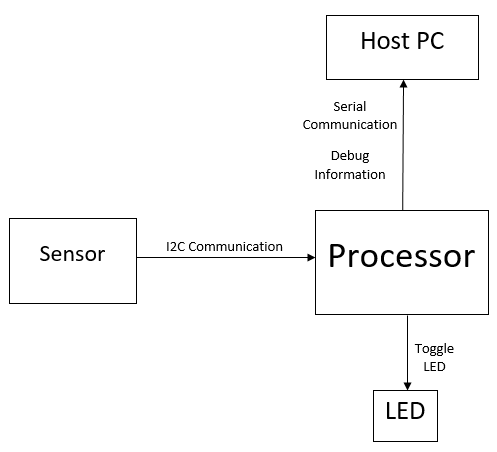
\includegraphics{hardware-schematics-development-2.pdf}
	\caption{Final Hardware Block Diagram - Development}
	\label{fig:hardware_schematic_development-2}
\end{figure}

\begin{figure}
	\centering
	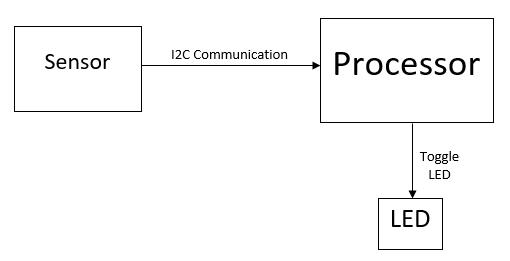
\includegraphics{hardware-schematics-final-2.pdf}
	\caption{Final Hardware Block Diagram - Final}
	\label{fig:hardware_schematic_final-2}
\end{figure}